\documentclass[tikz,border=5mm]{standalone}
\usepackage{tikz}
\usetikzlibrary{positioning,shapes,arrows.meta}

\begin{document}
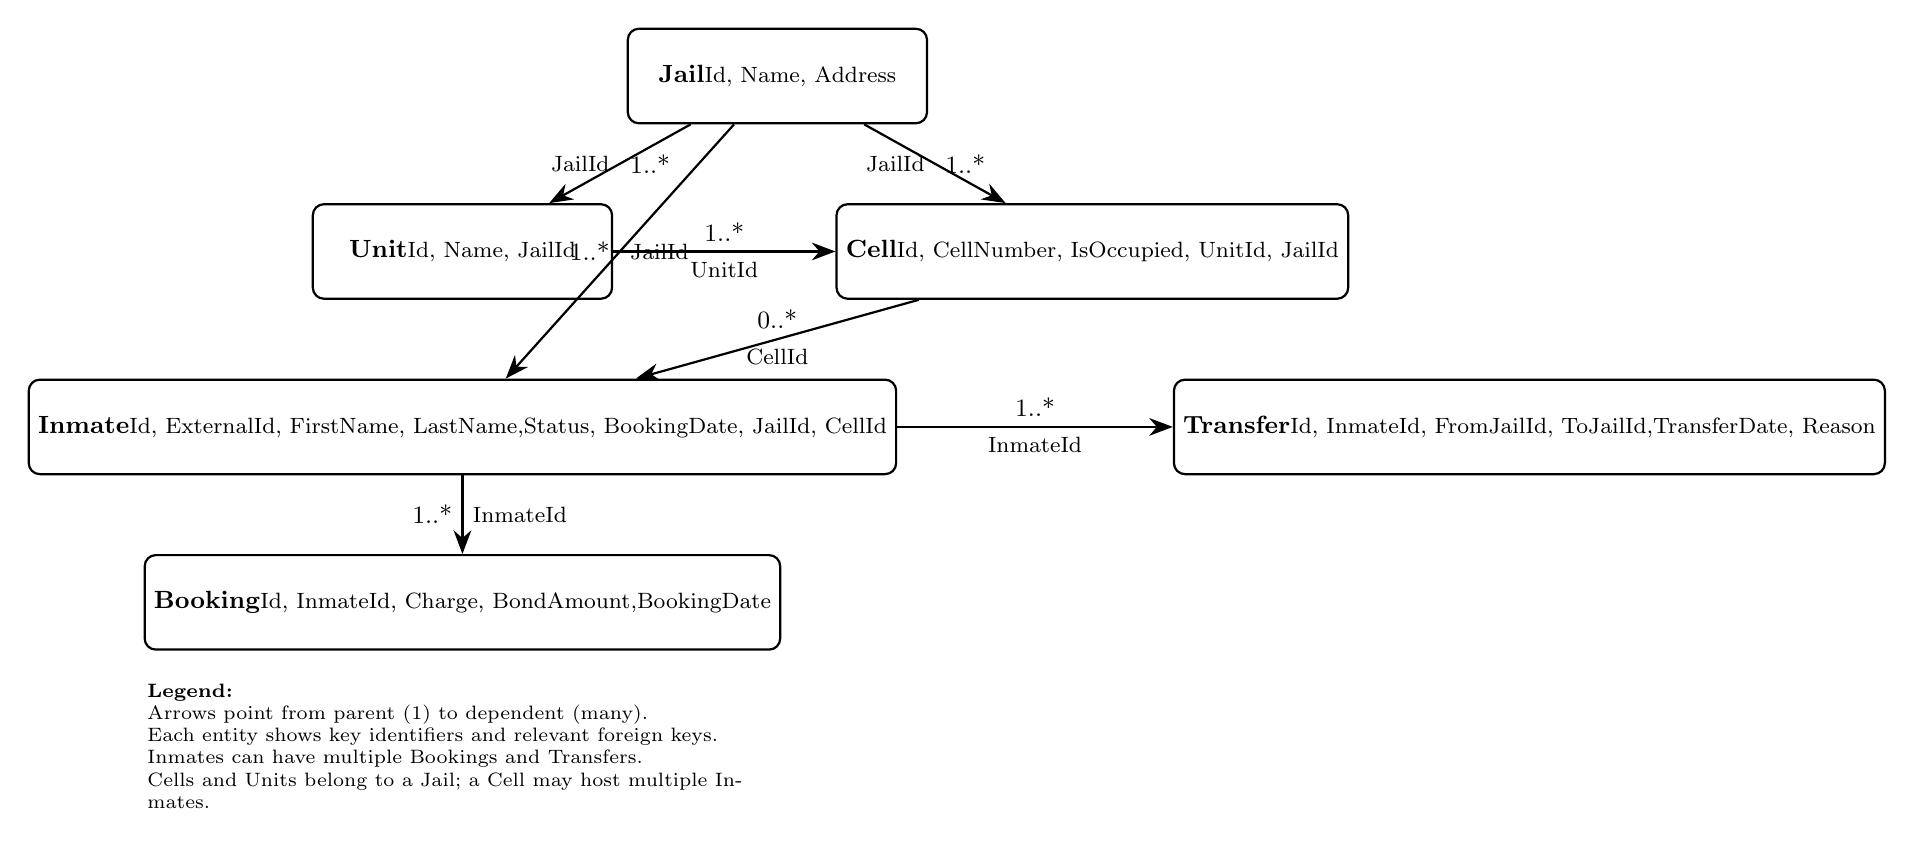
\begin{tikzpicture}[
  entity/.style={rectangle, draw=black, thick, fill=white, rounded corners,
                 text centered, minimum width=3.8cm, minimum height=1.2cm},
  relation/.style={draw, -{Stealth[length=3mm]}, thick},
  attrib/.style={ellipse, draw, fill=white, inner sep=1pt, font=\footnotesize},
  every node/.style={font=\small}
]

% ==========================================================
% Entities
% ==========================================================
\node[entity] (Jail) {\textbf{Jail}\\\footnotesize Id, Name, Address};
\node[entity, below=of Jail, xshift=-4cm] (Unit) {\textbf{Unit}\\\footnotesize Id, Name, JailId};
\node[entity, below=of Jail, xshift=4cm] (Cell) {\textbf{Cell}\\\footnotesize Id, CellNumber, IsOccupied, UnitId, JailId};
\node[entity, below=of Unit] (Inmate) {\textbf{Inmate}\\\footnotesize Id, ExternalId, FirstName, LastName,\\Status, BookingDate, JailId, CellId};
\node[entity, right=of Inmate, xshift=2.5cm] (Transfer) {\textbf{Transfer}\\\footnotesize Id, InmateId, FromJailId, ToJailId,\\TransferDate, Reason};
\node[entity, below=of Inmate] (Booking) {\textbf{Booking}\\\footnotesize Id, InmateId, Charge, BondAmount,\\BookingDate};

% ==========================================================
% Relationships
% ==========================================================
\draw[relation] (Jail) -- node[right]{1..*} node[left]{\footnotesize JailId} (Unit);
\draw[relation] (Jail) -- node[right]{1..*} node[left]{\footnotesize JailId} (Cell);
\draw[relation] (Unit) -- node[above]{1..*} node[below]{\footnotesize UnitId} (Cell);
\draw[relation] (Jail) -- node[left]{1..*} node[right]{\footnotesize JailId} (Inmate);
\draw[relation] (Cell) -- node[above]{0..*} node[below]{\footnotesize CellId} (Inmate);
\draw[relation] (Inmate) -- node[above]{1..*} node[below]{\footnotesize InmateId} (Transfer);
\draw[relation] (Inmate) -- node[left]{1..*} node[right]{\footnotesize InmateId} (Booking);

% ==========================================================
% Notes
% ==========================================================
\node[below=0.3cm of Booking, align=left, font=\scriptsize, text width=8cm] (legend) {
\textbf{Legend:}\\
Arrows point from parent (1) to dependent (many).\\
Each entity shows key identifiers and relevant foreign keys.\\
Inmates can have multiple Bookings and Transfers.\\
Cells and Units belong to a Jail; a Cell may host multiple Inmates.
};

\end{tikzpicture}
\end{document}
